\documentclass[12pt, letter]{exam}
\usepackage[utf8]{inputenc}
\usepackage[T1]{fontenc}
\usepackage[spanish]{babel}
\usepackage{amsmath}
\usepackage{amsthm}
\usepackage{physics}
\usepackage{tikz}
\usepackage{float}
\usepackage{siunitx}
\usepackage{multicol}
\usepackage[left=2.00cm, right=2.00cm, top=2.00cm, 
     bottom=2.00cm]{geometry}
\usepackage{pdfpages}
\usepackage{enumitem}
\usepackage{circuitikz}

% \renewcommand{\questionlabel}{\thequestion}
\decimalpoint

\setlength{\belowdisplayskip}{-0.5pt}

\usepackage{tasks}
\settasks{
    label=\Alph*), 
    label-align=left,
    item-indent={20pt}, 
    column-sep={4pt},
    label-width={16pt},
}

\sisetup{per-mode=symbol}
\footer{}{\thepage}{}

\begin{document}

\includepdf[pages=-]{Caratula_Examen_Ordinario_Fisica_4.pdf}
\setcounter{page}{3}

\newpage
\begin{center}
\textbf{Cada ejercicio vale 1 punto, incluidos los de ejecución.}
\end{center}

\begin{questions}

    \section{(4 puntos) Ondas.}
    
    \vbox{\leftskip\leftmargin A continuación se te presenta la definición de un concepto, la palabra faltante está en una de las opciones de respuesta, relaciona cada definición con la palabra.}

    \question Es el tiempo que se necesita para hacer una oscilación completa: \rule{2cm}{0.1mm}. 
    \begin{tasks}(4)
        \task Periodo
        \task Frecuencia
        \task Elongación
        \task Amplitud
    \end{tasks}
    \question Cuando se habla de la distancia que separa dos puntos equivalentes consecutivos de la onda, estamos haciendo referencia a \rule{2cm}{0.1mm} 
    \begin{tasks}(4)
        \task Amplitud
        \task Longitud de onda
        \task Cresta
        \task Periodo
    \end{tasks}
    \question \rule{2cm}{0.1mm} es el número de oscilaciones o vibraciones que realiza la onda por segundo.
    \begin{tasks}(4)
        \task Amplitud
        \task Longitud de onda
        \task Frecuencia
        \task Periodo
    \end{tasks}
    \question \label{Ejercicio_01} \textbf{Ejercicio de ejecución.} En una cuerda tensa se producen ondas con una frecuencia de \SI{240}{\hertz}, a una velocidad de propagación cuya magnitud es de \SI{150}{\meter\per\second}. ¿Qué longitud de onda tienen?
    \begin{tasks}(4)
       \task \SI{0.625}{\meter}
       \task \SI{0.855}{\meter}
       \task \SI{1.920}{\meter}
       \task \SI{1.102}{\meter}
   \end{tasks}
    % \question Cuando se habla de que es el recorrido de la onda desde un punto hasta el siguiente punto equivalente, se está hablando de: \rule{1.5cm}{0.1mm}
    % \begin{tasks}(4)
    %     \task Elongación.
    %     \task Cresta.
    %     \task Ciclo.
    %     \task Valle.
    % \end{tasks}
    % \question Se definen las ondas longitudinales a aquellas que se generan cuando las partículas del medio material vibra de manera \rule{2cm}{0.1mm} a la dirección de propagación de la onda.
    % \begin{tasks}(4)
    %     \task Uniforme
    %     \task Perpendicular
    %     \task Reflejante
    %     \task Paralela
    % \end{tasks}

    \section{(3 puntos) Fenómenos sonoros.}

    \question La \rule{2cm}{0.1mm} de las ondas se presenta cuando éstas encuentran un obstáculo que les impide propagarse.
    \begin{tasks}(4)
        \task Reflexión
        \task Refracción
        \task Compresión
        \task Rarefacción
    \end{tasks}
    \question Las ondas \rule{2cm}{0.1mm} se presenta cuando las partículas del medio material vibran paralelamente a la dirección de propagación de la onda.
    \begin{tasks}(4)
        \task Transversales
        \task Longitudinales
        \task Comprimidas
        \task Estacionarias
    \end{tasks}
    \question Es el nombre que se le da al desplazamiento que experimenta una partícula vibrante, equivalente a la suma vectorial de los desplazamientos que cada onda le produce.
    \begin{tasks}(4)
        \task Compresión
        \task Rarefacción
        \task Superposición.
        \task Expansión.
    \end{tasks}

    \section{(3 puntos) Oído.}

    \question Cuando la frecuencia de una onda sonora es inferior al límite audible, se dice que es \rule{2cm}{0.1mm}
    \begin{tasks}(4)
        \task Infrasónica
        \task Ultrasónica
        \task Hipersónica
        \task Ecosónica
    \end{tasks}
    
    % \question \textbf{Ejercicio de ejecución.} Determinar cuál es el periodo de las ondas producidas en una cuerda de violín si la velocidad de propagación tiene una magnitud de \SI{220}{\meter\per\second} y su longitud de onda es de $\lambda = \SI{0.2}{\meter}$.
    % \begin{tasks}(4)
    %    \task \SI{9.09d-2}{\second}
    %    \task \SI{9.09d-3}{\second}
    %    \task \SI{9.09d-4}{\second}
    %    \task \SI{9.09d-5}{\second}
    % \end{tasks}
%     \question \textbf{Ejercicio de ejecución.} Una fuente sonora produce un sonido con una frecuencia de \SI{750}{\hertz}, calcula su longitud de onda en el agua, considera que la magnitud de la velocidad del sonido en el agua es de \SI{1435}{\meter\per\second}.
%     \begin{tasks}(4)
%        \task \SI{1.813}{\meter}
%        \task \SI{1.913}{\meter}
%        \task \SI{2.856}{\meter}
%        \task \SI{3.102}{\meter}
%    \end{tasks}
   \question \label{Ejercicio_02} \textbf{Ejercicio de ejecución.} ¿Cuál es la intensidad de un sonido de \SI{40}{\dB}?
   \begin{tasks}(4)
       \task \SI{1d-8}{\watt\per\square\meter}
       \task \SI{1d-9}{\watt\per\square\meter}
       \task \SI{1d-10}{\watt\per\square\meter}
       \task \SI{1d-11}{\watt\per\square\meter}
   \end{tasks}
   \question \label{Ejercicio_03} \textbf{Ejercicio de ejecución.} La conversación ordinaria corresponde a un nivel de sonido de aproximadamente \SI{65}{\dB}. Si dos personas hablan al mismo tiempo, el nivel de sonido es:
   \begin{tasks}(4)
       \task \SI{65}{\dB}
       \task \SI{68}{\dB}
       \task \SI{75}{\dB}
       \task \SI{130}{\dB}
   \end{tasks}

   \section{(2 puntos) Efecto Doppler.}

   \question \label{Ejercicio_04} \textbf{Ejercicio de ejecución: } Una ambulancia lleva una velocidad cuya magnitud es de \SI{70}{\kilo\meter\per\hour} y su sirena suena con una frecuencia de \SI{830}{\hertz}. ¿Qué frecuencia aparente escucha un observador que está parado, cuando la ambulancia se aleja de él? Considera que la velocidad del sonido en el aire es de \SI{340}{\meter\per\second}.
   \begin{tasks}(4)
    \task \SI{785.11}{\hertz}
    \task \SI{880.33}{\hertz}
    \task \SI{1000.00}{\hertz}
    \task \SI{1659.19}{\hertz}
    \end{tasks}
    \question \label{Ejercicio_05} \textbf{Ejercicio de ejecución: } Un automovilista que viaja a una velocidad cuya magnitud es de \SI{80}{\kilo\meter\per\hour} escucha el silbato de una fábrica cuya frecuencia es de \SI{1100}{\hertz}. Calcula la frecuencia aparente escuchada por el automovilista cuando se acerca a la fuente. Considera que la velocidad del sonido en el aire es de \SI{340}{\meter\per\second}
    \begin{tasks}(4)
        \task \SI{899.20}{\hertz}
        \task \SI{1171.88}{\hertz}
        \task \SI{1905.07}{\hertz}
        \task \SI{2416.23}{\hertz}
    \end{tasks}

    \section{(1 punto) Óptica geométrica.}

    \question ¿Cuáles son las características de la luz que se cumplen tanto en la teoría corpuscular de la luz y la teoría ondulatoria?
    {\renewcommand{\thepartno}{\Alph{partno}}
    \begin{parts}
        \part Refracción, Reverberación, Reflexión.
        \part Reflexión, Resonancia, Propagación rectilínea.
        \part Propagación rectilínea, Reflexión, Refracción.
        \part Refracción, Efecto Doppler, Reflexión.
    \end{parts}
    }

    \newpage

    \section{(2 puntos) Refracción.}

    \question De la ley de Snell se nos pide obtener el ángulo $b$ (refractado), ¿Cuál es la expresión que nos resuelve el problema?
    \begin{multicols}{2}
    \begin{tasks}
        \task $ b = \sen^{-1} \left(\dfrac{n_{b} \, \text{sen} \, a}{n_{a}} \right)$
        \task $ b = \sen^{-1} \left(\dfrac{n_{a} \, \text{sen} \, a}{n_{b}} \right)$
        \task $ b = \sen^{-1} \left(\dfrac{n_{a} \, n_{b}}{\text{sen} \, a} \right)$
        \task $ b = \sen^{-1} \left(\dfrac{\text{sen} \, a}{n_{a} \, n_{b}} \right)$
    \end{tasks}
    \end{multicols}
    \question \label{Ejercicio_06} \textbf{Ejercicio de ejecución: } El haz de una linterna incide sobre la superficie de un panel de vidrio $(n_{v} = 1.56)$ en un ángulo de \ang{75} con la normal. ¿Cuál es el ángulo de refracción? El índice de refracción del aire es $n_{a} = 1.0$
    \begin{tasks}(4)
        \task \ang{27.19}
        \task \ang{39.83}
        \task \ang{38.25}
        \task \ang{48.07}
    \end{tasks}

    \section{(5 puntos) Lentes delgadas.}

    \question Las lentes \rule{2.5cm}{0.1mm} son aquellas cuyo espesor disminuye de los bordes hacia el centro, hablamos de las lentes:
    \begin{tasks}(4)
        \task Esféricas.
        \task Divergentes.
        \task Convergentes.
        \task Cilíndricas.
    \end{tasks}
    \question Revisa con cuidado la siguiente imagen e identifica las siguientes lentes en el orden que se presenta, ya sean positivas (+) o negativas (-).
    \begin{figure}[H]
        \centering
        
\includegraphics[scale=2]{Imagenes/Arreglo_Lentes_02.png}
    \end{figure}
    \begin{tasks}(4)
        \task \textbf{+, - , +, -}
        \task \textbf{-, - , +, +} 
        \task \textbf{+, + , -, -} 
        \task \textbf{-, + , -, +} 
    \end{tasks}
    \question De la convención de signos para las lentes delgadas:  La distancia de la imagen $d_{i}$ es \rule{2cm}{0.1mm} para una imagen virtual.
    \begin{tasks}(4)
        \task Negativa.
        \task Positiva.
        \task Infinita.
        \task Cero.
    \end{tasks}
    \question \label{Ejercicio_07} \textbf{Ejercicio de ejecución. } Un objeto de \SI{15}{\centi\meter} se coloca a \SI{50}{\centi\meter} de una lente positiva que tiene una distancia focal de \SI{20}{\centi\meter}. ¿De qué tamaño es la imagen?

    \vspace{0.3cm}
    \begin{tasks}(4)
        \task \textbf{+}\SI{19.85}{\centi\meter}
        \task \textbf{+}\SI{25.20}{\centi\meter}
        \task \SI{-5.04}{\centi\meter}
        \task \SI{-9.99}{\centi\meter}
    \end{tasks}
    \question \label{Ejercicio_08} \textbf{Ejercicio de ejecución: } ¿Cuál es la potencia de una lente con \SI{15}{\centi\meter} de distancia focal?
    \begin{tasks}(4)
        \task \num{-2.98} Dioptrías
        \task \num{2.98} Dioptrías
        \task \num{6.66} Dioptrías
        \task \num{-5.25} Dioptrías
    \end{tasks}

    \section{(2 puntos) Defectos de la visión.}
    
    \question El siguiente esquema representa un ojo humano, ¿cómo se denomina al caso en términos de anomalías/normalidad de la visión?
    \begin{figure}[H]
        \centering
        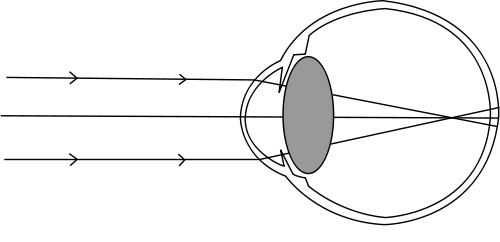
\includegraphics[scale=0.3]{Imagenes/Defectos_Vision_03.png}
    \end{figure}
    \begin{tasks}(4)
        \task Ojo astigmata.
        \task Ojo emétrope.
        \task Ojo hipermétrope.
        \task Ojo miope.
    \end{tasks}
    \question  La \rule{2cm}{0.1mm} es la capacidad de utilizar ambos ojos de manera coordinada y simultánea para percibir una sola imagen tridimensional del entorno.
    \begin{tasks}(4)
        \task Visión periférica.
        \task Visión 20/20.
        \task Visión monocular.
        \task Visión binocular.
    \end{tasks}

    \section{(1 puntos) Ecuación de continuidad.}

    \question En la hidrodinámica un fluido se considera ideal cuando \rule{2cm}{0.1mm}:
    \begin{tasks}
        \task La densidad del fluido es variable.
        \task Las fuerzas son no conservativas.
        \task El fluido es irrotacional.
        \task La temperatura del fluido varía con la velocidad.
    \end{tasks}

    \section{(2 puntos) Ecuación de Bernoulli.}

    \question \label{Ejercicio_09} \label{Problema_01} \textbf{Ejercicio de ejecución: } En el cuerpo humano el flujo sanguíneo es de $5$ litros de sangre por minuto. ¿Cuál es el área de la sección transversal de la aorta, si la sangre en ese vaso tiene una velocidad de \SI{28}{\centi\meter\per\second}? Recuerda que 1 litro = \SI{1000}{\cubic\centi\meter}.
    \begin{tasks}(4)
        \task \SI{2.77}{\square\centi\meter}
        \task \SI{2.97}{\square\centi\meter}
        \task \SI{3.10}{\square\centi\meter}
        \task \SI{1.77}{\square\centi\meter}
    \end{tasks}
%     \question \textbf{(1 punto)} Bernoulli al estudiar la relación entre la presión y la velocidad de un líquido que circula por una tubería, encontró que la presión es \rule{2cm}{0.1mm} si su velocidad es \rule{2cm}{0.1mm}:
%     \begin{tasks}(4)
%         \task alta - cero.
%         \task baja - máxima.
%         \task baja - alta.
%         \task alta - alta.
%     \end{tasks}
%     \question \textbf{(1 punto)} La ecuación de Bernoulli que se muestra a continuación contiene tres términos de cada lado de la igualdad:
%     \begin{align*}
%     \underbrace{P_{1}}_{\text{\large{a}}} + \underbrace{\rho \, g \, h_{1}}_{\text{\large{b}}} + \underbrace{\dfrac{1}{2} \rho \, v_{1}^{2}}_{\text{\large{c}}} = P_{2} + \rho \, g \, h_{2} + \dfrac{1}{2} \rho \, v_{2}^{2}
%     \end{align*}
        
%     \vspace{0.5em}
%     \begin{inparaenum}[I)]
%             \item Energía cinética. \quad \quad
%             \item Energía potencial. \quad \quad
%             \item Potencia. \quad \quad
%             \item Presión.
%     \end{inparaenum}

%     Selecciona la respuesta que relaciona los tres términos con las cantidades físicas correspondientes.
%     \begin{tasks}
%         \task a - III, b - I, c - II
%         \task a - IV, b - I, c - II
%         \task a - IV, b - II, c - I
%         \task a - III, b - II, c - I
%     \end{tasks}
    \question En la siguiente figura se presenta el flujo \rule{2cm}{0.1mm} en un conducto.
    \begin{figure}[H]
        \centering
        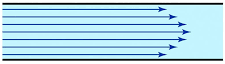
\includegraphics[scale=0.8]{Imagenes/Flujo_02_Laminar.png}
    \end{figure}
    \begin{tasks}(4)
        \task laminar
        \task turbulento
        \task seccionado
        \task estático
    \end{tasks}
%     \question \textbf{(1 punto)} El número de Reynolds es una cantidad adimensional que nos indica cuándo un flujo \rule{2cm}{0.1mm} pasa a ser un flujo \rule{2cm}{0.1mm}.
%     \begin{tasks}
%         \task laminar - seccionado
%         \task estático - turbulento
%         \task laminar  - turbulento
%         \task turbulento - laminar
%     \end{tasks}
    
    \section{(2 puntos) Corriente directa y alterna.}

    \question El flujo de las partículas cargadas en un conductor es lo que se conoce como \rule{2cm}{0.1mm}.
    \begin{tasks}(4)
        \task Resistencia.
        \task Voltaje.
        \task Potencia.
        \task Corriente.
    \end{tasks}
    \question Relaciona las siguientes cantidades con las respectivas unidades, una columna con la otra.
    
    \begin{minipage}[t]{0.4\linewidth}
        \begin{enumerate}[label=\arabic*)]
            \item Voltaje.
            \item Resistencia.
            \item Corriente.
        \end{enumerate}
    \end{minipage}
    \begin{minipage}[t]{0.4\linewidth}
        \begin{enumerate}[label=\alph*)]
            \item Ohm (\unit{\ohm})
            \item Watt (\unit{\watt})
            \item Ampere (\unit{\ampere})
            \item Volt (\unit{\volt})
        \end{enumerate}
    \end{minipage}
    \begin{tasks}(4)
        \task 1-d, 2-b, 3-a
        \task 1-a, 2-d, 3-c
        \task 1-d, 2-a, 3-c
        \task 1-a, 2-c, 3-b
    \end{tasks}

    \section{(2 puntos) Ley de Ohm.}

    \question \label{Ejercicio_10} \label{Problema_02} \textbf{Ejercicio de ejecución: } Determina la intensidad de la corriente eléctrica a través de una resistencia de \SI{150}{\kilo\ohm} al aplicarle una diferencia de potencial de \SI{220}{\volt}.
    \begin{tasks}(4)
        \task \SI{1.466}{\milli\ampere}
        \task \SI{1.966}{\ampere}
        \task \SI{2.066}{\milli\ampere}
        \task \SI{2.066}{\ampere}
    \end{tasks}
    \question \label{Ejercicio_11} \label{Problema_03} \textbf{Ejercicio de ejecución: } Calcula la diferencia de potencial aplicada a una resistencia de \SI{20}{\ohm} y por ella fluyen \SI{12}{\ampere}.
    \begin{tasks}(4)
        \task \SI{200}{\volt}
        \task \SI{220}{\volt}
        \task \SI{240}{\volt}
        \task \SI{300}{\volt}
    \end{tasks}

    \section{(3 puntos) Circuitos eléctricos.}

    \question En el siguiente circuito eléctrico se tienen $n$ resistencias del mismo valor conectadas en serie, ¿cuál es el valor de la resistencia total $(R_{T})$ del circuito entre los puntos $A^{\prime}$ y $B^{\prime}$?
    \begin{center}
    \begin{circuitikz}[american voltages]
        \draw 
            (0, 0) node [anchor=east] {$A^{\prime}$}
            to[short, o-] (1, 0)
            % (0, 0) to[V=10V] (0, 4)
            to [R, l=\mbox{$R$}] (3, 0)
            to [R, l=\mbox{$R$}] (5, 0)
            to [R, l=\mbox{$R$}] (7, 0)
            -- (8.5, 0) node[midway,fill=white,inner sep=5,scale=1.2] {$.\,.\,.$} (10.5, 0)
            ;
            \draw (8.5, 0) to [R, l=\mbox{$R$}] (10.5, 0)
                to[short, -o] (12, 0)
                node [anchor=west] {$B^{\prime}$};
    \end{circuitikz}  
    \end{center}
    \begin{tasks}(4)
        \task $R_{T} = n^{2} \, R$
        \task $R_{T} = n + R$
        \task $R_{T} = n \, R$
        \task $R_{T} = \dfrac{R}{n}$
    \end{tasks}
    \question En un circuito $RC$ en serie, se tiene que $R = \SI{5}{\kilo\ohm}$ y $C = \SI{3}{\micro\farad}$. ¿Cuál es la constante de tiempo del circuito?
    \begin{tasks}(4)
        \task \SI{1.5d-3}{\second}
        \task \SI{0.015}{\second}
        \task \SI{15}{\second}
        \task \SI{0.35}{\second}
    \end{tasks}
%     \question \textbf{(1 punto)} En un circuito \rule{2cm}{0.1mm} la corriente se adelanta \ang{90} con respecto al voltaje:
%     \begin{tasks}(4)
%         \task $R \, C$
%         \task $R \, L$
%         \task $R \, L \, C$
%         \task $R$
%     \end{tasks}
    \question \label{Ejercicio_12} \label{Problema_05} \textbf{Ejercicio de ejecución: } Calcula la reactancia inductiva del siguiente inductor:
    \begin{center}
        \begin{circuitikz}[american voltages]
            \draw 
                (0, 0) to[short, o-] (1, 0)
                to [L, l=\mbox{$L=\SI{1.2}{\henry}$}] (3, 0)
                to[short, -o] (4, 0);
            \node at (2, -0.75) {$\omega = \SI{377}{\radian\per\second}$};
        \end{circuitikz}  
    \end{center}
    \begin{tasks}(4)
        \task \SI{246.1}{\ohm}
        \task \SI{370.7}{\ohm}
        \task \SI{452.4}{\ohm}
        \task \SI{500.9}{\ohm}
    \end{tasks}

    \section{(1 punto) Impedancia eléctrica.}

    % \question \textbf{(1 punto)} En un circuito en serie una resistencia $R = \SI{8}{\ohm}$ y un inductor $L = \SI{0.02}{\henry}$ están conectados a una fuente de voltaje $v = \num 283 \, \sin 300 \, t$ Volts. ¿Cuál es el valor de la impedancia compleja?
    % \begin{tasks}(4)
    %     \task $Z {=} \SI{16}{\ohm} + j \, \SI{16}{\ohm}$
    %     \task $Z {=} \SI{16}{\ohm} - j \, \SI{16}{\ohm}$
    %     \task $Z {=} \SI{8}{\ohm} - j \, \SI{6}{\ohm}$
    %     \task $Z {=} \SI{8}{\ohm} + j \, \SI{6}{\ohm}$
    % \end{tasks}
    \question \label{Ejercicio_13} \textbf{Ejercicio de ejecución: } Una resistencia $R = \SI{27.5}{\ohm}$ y un capacitor $C = \SI{66.7}{\micro\farad}$ se conectan en serie. La diferencia de potencial es $V = \num{50} \, \cos 1500 \, t$ \, Volts. ¿Cuál es la magnitud de la impedancia eléctrica $Z$?
    \begin{tasks}(4)
        \task \SI{14.99}{\ohm}
        \task \SI{980.95}{\ohm}
        \task \SI{29.26}{\ohm}
        \task \SI{224.70}{\ohm}
    \end{tasks}

    \section{(5 puntos) Instrumentación biomédica.}

    \question El estetoscopio Pinard es un tipo de instrumento de diagnóstico que se clasifica en el grupo de estetoscopios: \rule{2cm}{0.1mm}
    \begin{tasks}(4)
        \task Automático.
        \task Electrónico.
        \task Mecánico.
        \task Estándar.
    \end{tasks}
    \question Con el esfigmomanómetro se registran dos valores de presión arterial, el primero y más alto corresponde a la presión: \rule{2cm}{0.1mm}
    \begin{tasks}(4)
        \task Intraarticular.
        \task Sistólica.
        \task Diastólica.
        \task Abdominal.
    \end{tasks}
    \question El inicio de los ruidos de Korotkoff se presenta cuando la presión \rule{2cm}{0.1mm} es \rule{2cm}{0.1mm} que la presión del brazalete del esfigmomanómetro.
    \begin{multicols}{2}
    \begin{tasks}
        \task Sistólica - Mayor
        \task Diastólica - Mayor
        \task Diastólica - Menor
        \task Sistólica - Menor
    \end{tasks}
    \end{multicols}
    \question Es el tipo de radiación ionizante que se utiliza en equipos de tomografía axial computarizada: \rule{2cm}{0.1mm}
    \begin{multicols}{2}
    \begin{tasks}
        \task Rayos Ultravioleta.
        \task Rayos X.
        \task Rayos Infrarrojos.
        \task Rayos Gamma.
    \end{tasks}
    \end{multicols}
    \question Con un equipo de ultrasonido se envían ondas sonoras al cuerpo, el fenómeno que se presenta entre las ondas y el cuerpo es la \rule{2cm}{0.1mm}, que permite el registro y reconstrucción en una imagen bidimensional de la zona anatómica.
    \begin{tasks}(4)
        \task Refracción
        \task Reflexión
        \task Rarefacción
        \task Compresión
    \end{tasks}

    \section{(2 puntos) Potencial de acción.}

    \question Cuando hablamos de la diferencia en las concentraciones iónicas a nivel intra y extracelular, que condiciona una diferencia entre las cargas a ambos lados de la membrana, las mismas que tratarán de igualarse, hablamos del equilibrio de: \rule{2cm}{0.1mm}
    \begin{tasks}(4)
        \task Hodgkin
        \task Huxley
        \task Goldman-Katz
        \task Gibbs-Donnan
    \end{tasks}
    \question Se presenta a continuación una gráfica del potencial de acción, relaciona las fases (inciso con minúsculas) con un número romano en la gráfica.
    \begin{figure}[H]
        \centering
        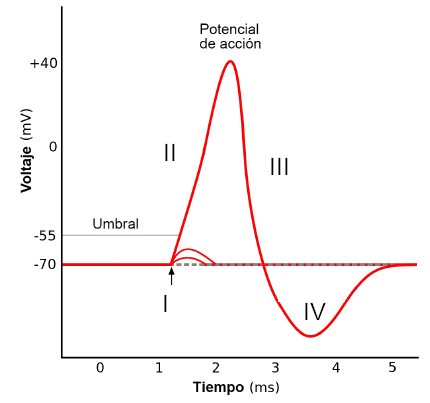
\includegraphics[scale=0.75]{Imagenes/Potencial_Accion_07.png}
    \end{figure}

    Fases del potencial de acción:
    \renewcommand{\thepartno}{\alph{partno}}
    \begin{multicols}{2}
    \begin{parts}
        \part Estímulo
        \part Reposo
        \part Repolarización
        \part Período refractario
        \part Despolarización
         \vspace*{\fill}
    \end{parts}
    \end{multicols}

    Opciones de respuesta:
    \begin{multicols}{2}
    \begin{tasks}
        \task I-a, II-d, III-b, IV-e
        \task I-e, II-b, III-d, IV-c
        \task I-a, II-e, III-c, IV-d
        \task I-a, II-e, III-c, IV-b
    \end{tasks}
    \end{multicols}

\end{questions}

\newpage

% \vspace*{1cm}
\textbf{\huge{Formulario.}}
\begin{table}[H]
    \centering
    \setlength{\tabcolsep}{40pt}
    \renewcommand{\arraystretch}{2.5}
    \begin{tabular}{c  c}
        \multicolumn{2}{c}{Ondas} \\
        $v = \lambda \, f$ & $T = \dfrac{1}{f}$ \\ \hline
        \multicolumn{2}{c}{Sonido} \\
        $B = 10 \, \log \left( \dfrac{I}{I_{0}} \right)$ & $I_{0} = \SI{1d-12}{\watt\per\square\meter}$ \\
        $\lambda = \dfrac{2 \, L}{n}$ & $f^{\prime} = \dfrac{f \, V}{V \pm v}$ \\
        $f^{\prime} = \dfrac{f \, (V \pm v)}{v}$ & \\ \hline
        \multicolumn{2}{c}{Óptica geométrica} \\
        $n = \dfrac{\text{sen} \, i}{\text{sen} \, i}$ & $n_{a} \, \text{sen} \,  a = n_{b} \, \text{sen} \,  b$ \\ \hline
        \multicolumn{2}{c}{Lentes delgadas} \\
        $\dfrac{1}{f} = \dfrac{1}{d_{o}} + \dfrac{1}{d_{i}}$ (lente convergente) & $- \dfrac{1}{f} = \dfrac{1}{d_{o}} - \dfrac{1}{d_{i}}$ (lente divergente) \\
        $m = - \dfrac{d_{i}}{d_{o}} = \dfrac{h_{i}}{h_{o}}$ & $\text{Potencia } = \dfrac{1}{f} \quad f \text{ en } \unit{\meter}$ \\ \hline
        \multicolumn{2}{c}{Hidrodinámica} \\
        $G = \dfrac{V}{t}$ & $G = A \, v$ \\
        $\text{Flujo} = \dfrac{m}{t}$ & $\text{Flujo} = \dfrac{\rho \, V}{t}$ \\
        $\text{Flujo} = G \, \rho$ & \\
        $v_{1} \, A_{1} = v_{2} \, A_{2}$ & $v = \sqrt{2 \, g \, h}$ \\
        \multicolumn{2}{c}{$P_{1} + \rho \, g \, h_{1} + \dfrac{1}{2} \rho \, v_{1}^{2} = P_{2} + \rho \, g \, h_{2} + \dfrac{1}{2} \rho \, v_{2}^{2}$}
    \end{tabular}
\end{table}

\newpage

\begin{table}[H]
    \centering
    \setlength{\tabcolsep}{40pt}
    \renewcommand{\arraystretch}{2.5}
    \begin{tabular}{c  c}
        \multicolumn{2}{c}{Electricidad} \\
        $V = I \, R$ & $R_{T} = R_{1} + R_{2} + R_{3} + \ldots$ \\
        $\dfrac{1}{R_{T}} = \dfrac{1}{R_{1}} + \dfrac{1}{R_{2}} + \dfrac{1}{R_{3}} + \ldots$ & $\tau = R \, C$ \\
        $X_{C} = \dfrac{1}{\omega \, C}$ & $X_{L} = \omega\, L$ \\
        $Z = R + j \, X_{L}$ & $Z = R - j \, X_{C}$ \\
        $\abs{Z} = \sqrt{R^{2} + (X_{L})^{2}}$ & $\abs{Z} = \sqrt{R^{2} + (X_{C})^{2}}$ \\
        $Z = R + j (X_{L} - X_{C})$ & $\abs{Z} = \sqrt{R^{2} + (X_{L} - X_{C})^{2}}$
\end{tabular}
\end{table}

\newpage

En este espacio deberás de incluir el desarrollo completo de los Problemas de Ejecución. El problema se califica de la siguiente manera: \textbf{a) Datos: 0.25 puntos}, \textbf{b) Expresión(es): 0.25 puntos}, \textbf{c) Sustitución: 0.25 puntos} y \textbf{d) Manejo de unidades: 0.25 puntos}.

\vspace*{0.5cm}
Solución al Problema de Ejecución \ref{Ejercicio_01}:

\vspace*{4cm}
\rule{0.9\textwidth}{0.1mm}

Solución al Problema de Ejecución \ref{Ejercicio_02}:

\vspace*{4.5cm}
\rule{0.9\textwidth}{0.1mm}

Solución al Problema de Ejecución \ref{Ejercicio_03}:

\vspace*{4.5cm}
\rule{0.9\textwidth}{0.1mm}

Solución al Problema de Ejecución \ref{Ejercicio_04}:

\vspace*{4.5cm}
\rule{0.9\textwidth}{0.1mm}

Solución al Problema de Ejecución \ref{Ejercicio_05}:

\vspace*{4.5cm}
\rule{0.9\textwidth}{0.1mm}

Solución al Problema de Ejecución \ref{Ejercicio_06}:

\vspace*{4.5cm}
\rule{0.9\textwidth}{0.1mm}

Solución al Problema de Ejecución \ref{Ejercicio_07}:

\vspace*{4.5cm}
\rule{0.9\textwidth}{0.1mm}

Solución al Problema de Ejecución \ref{Ejercicio_08}:

\vspace*{4.5cm}
\rule{0.9\textwidth}{0.1mm}

Solución al Problema de Ejecución \ref{Ejercicio_09}:

\vspace*{4.5cm}
\rule{0.9\textwidth}{0.1mm}

Solución al Problema de Ejecución \ref{Ejercicio_10}:

\vspace*{4.5cm}
\rule{0.9\textwidth}{0.1mm}

Solución al Problema de Ejecución \ref{Ejercicio_11}:

\vspace*{4.5cm}
\rule{0.9\textwidth}{0.1mm}

Solución al Problema de Ejecución \ref{Ejercicio_12}:

\vspace*{4.5cm}
\rule{0.9\textwidth}{0.1mm}

Solución al Problema de Ejecución \ref{Ejercicio_13}:


\end{document}